\chapter{Introduction}

Unmanned Aerial Vehicles (UAVs) have seen explosive growth in the past thirty years, performing a multitude of military and civilian tasks including surveillance, reconnaissance, armed combat operations, search and rescue, forest fire management, and domestic policing \cite{sarris2001survey, valavanis2007advances}. A class of modern UAVs which have recently grown in popularity are quadrotors -  Vertical Take Off and Landing (VTOL) vehicles powered by four rotors arranged in a cross or x configuration. The main advantage of the quadrotor lies in its mechanical simplicity. Adjusting the speed of one or more of the vehicle's fixed-pitch rotors provides full attitude control, eliminating the need for the swash plate mechanism found on single rotor helicopters \cite{bramwell2001bramwell, gupte2012survey}. In spite of its mechanical simplicity, the quadrotor exhibits complex nonlinear dynamics. Because they have only four independent inputs (motor speeds) to control six degrees of freedom (three translational and three rotational), quadrotors are underactuated systems that must be modeled as Multi-Input Multi-Output (MIMO) systems.
\begin{figure}[htb!]
	\centering
	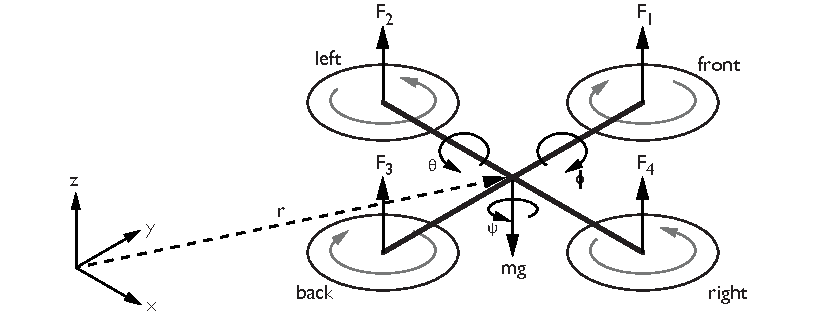
\includegraphics{../fig/quad.pdf}
	\caption[A quadrotor arranged in the cross configuration.]{A quadrotor arranged in the cross configuration. The position vector of the vehicle's center of mass relative to the inertial reference frame is $r$. Vehicle pitch is $\theta$, roll is $\phi$, and yaw is $\psi$. Motor forces $F_1$, $F_2$, $F_3$, and $F_4$ act upwards in the vehicle's body frame and the force of gravity acts downward in the inertial frame.}
\end{figure}


Advances in MEMS sensors and light-weight high-powered lithium polymer batteries have contributed to the recent popularity of quadrotors, making them an attractive choice for research applications in flight dynamics and control, as in \cite{hoffmann2007quadrotor, kivrak2006design, mellinger2010control, michael2010grasp}. One problem of particular interest is the development of mathematical models representing system dynamics based on experimentally gathered data. System identification provides a mechanism to relate this input-output data to the underlying system dynamics, without assuming any a priori knowledge of the system. Traditionally, system identification techniques have focused on developing a system model which minimizes prediction error. Identification methods of this form are commonly known as Prediction Error Methods (PEMs). PEMs have seen widespread use in both theoretical and real-world applications, but experience difficulties identifying MIMO systems as noted in \cite{qin2006overview, viberg1995subspace}. 

Subspace identification methods have recently grown in popularity and offer an alternative approach to the identification problem. These methods have a foundation in linear algebra and overcome some of the issues found in PEMs when identifying MIMO systems \cite{katayama2005subspace}. While traditional subspace algorithms provide reliable results when identifying systems operating in open loop, modifications must be made to identify systems operating in closed loop to eliminate a bias introduced by feedback control. It is the goal of this research project to apply subspace identification techniques using innovation estimation to a quadrotor using experimentally gathered closed-loop input and output data.


\section{Related Work}
Developing accurate dynamical models of quadrotors plays an important role in their development, test, and continuing operational use. Quadrotors are dynamically unstable and their dynamics are highly nonlinear. Developing system models from first principles is not commonly done due to the complexity of the resulting models and the difficulty of determining numerous unknown system parameters. Several groups have developed simple quadrotor models by directly measuring or estimating system parameters \cite{bresciani2008modelling, domingues2009quadrotor, kivrak2006design, pounds2006modelling, schreier2012modeling}, but these models are typically used to select initial controller gains during control system design, and full model simulation results are generally not given. 

Using prediction error techniques has proven to be viable approach to identifying quadrotor models from input-output data. In \cite{chamberlain2011system}, a system model is identified via an AutoRegressive model with external input (ARX) approach using position and attitude data measured by a Cortex 3D camera-based positioning system. NASA's System Identification Programs for Aircraft (SIDPAC) implementation of a least squares PEM is used to individually identify four dynamic modes of a quadcopter (lateral, longitudinal, heave, and yaw) in isolation in \cite{miller2011open} with output data measured by a Vicon motion capture system. Both cases showed accurate results when comparing predicted system output with measured system response. Model accuracy is boosted by the use of camera positioning systems to measure system position and attitude, which ensures the output data used for identification is free of some errors present in onboard sensor measurements caused by accelerometer drift and vehicle vibrations. When camera positioning systems are not available, it is still possible to identify models using measurements taken by onboard accelerometers and gyroscopes.  A model developed using prediction error in \cite{lee2011attitude} gave acceptable results when simulating pitch and roll dynamics but did not accurately model yaw dynamics.

Subspace identification techniques have also been shown to produce models which accurately describe quadrotor system dynamics. Motor dynamics were identified using numerical algorithms for subspace state space system identification (N4SID) in \cite{kis2011sensor} and the resulting model was used to simulate vehicle vertical acceleration. In \cite{batmazdesign}, N4SID was used to identify quadrotor roll dynamics from open-loop data collected by fixing all other vehicle degrees of freedom using a test bench setup. 


\section{Motivation and Contributions}
As subspace identification techniques continue to evolve, particularly in emerging areas of research including identification of systems in the presence of feedback control, demonstration of empirical results remains important to validate the real world usefulness and application of these theories. The motivation for the work presented here is to show empirical results from the development of dynamical models through subspace identification with innovation estimation. Specifically, we show that a six degree of freedom (6DOF) linear time-invariant (LTI) model of a quadrotor developed using innovation estimation provides an accurate representation of the true dynamical system.




